\documentclass{article}

\usepackage{algorithmic}
\usepackage{amsmath}
\usepackage{graphicx}
\usepackage{hyperref}
\usepackage{booktabs}

\begin{document}

\title{EM Algorithm}
\author{Geoffrey Ulman\\
        Homework 8\\
        CSI873}
\date{November 2011}
\maketitle

\section{Results}\label{Results}

Running the EM algorithm on the provided \(2000\) values (known to be drawn from two Gaussian distributions with variance 1.0) resulted in mean estimates of \(0.45\) and \(-0.74\). The evolution of the two mean estimates as the EM algorithm progressed is plotted in Figure \ref{fig1}. A histogram of the full data set is provided in Figure \ref{fig2} as a sanity check.

Java (version 1.6.0\_27) was used to implement the EM algorithm. The code is available as a Subversion repository on Google Code at \url{http://code.google.com/p/csi873/}. Compiling and running the code requires the Java build tool Maven (\url{http://maven.apache.org/}).

\begin{figure}
\centering
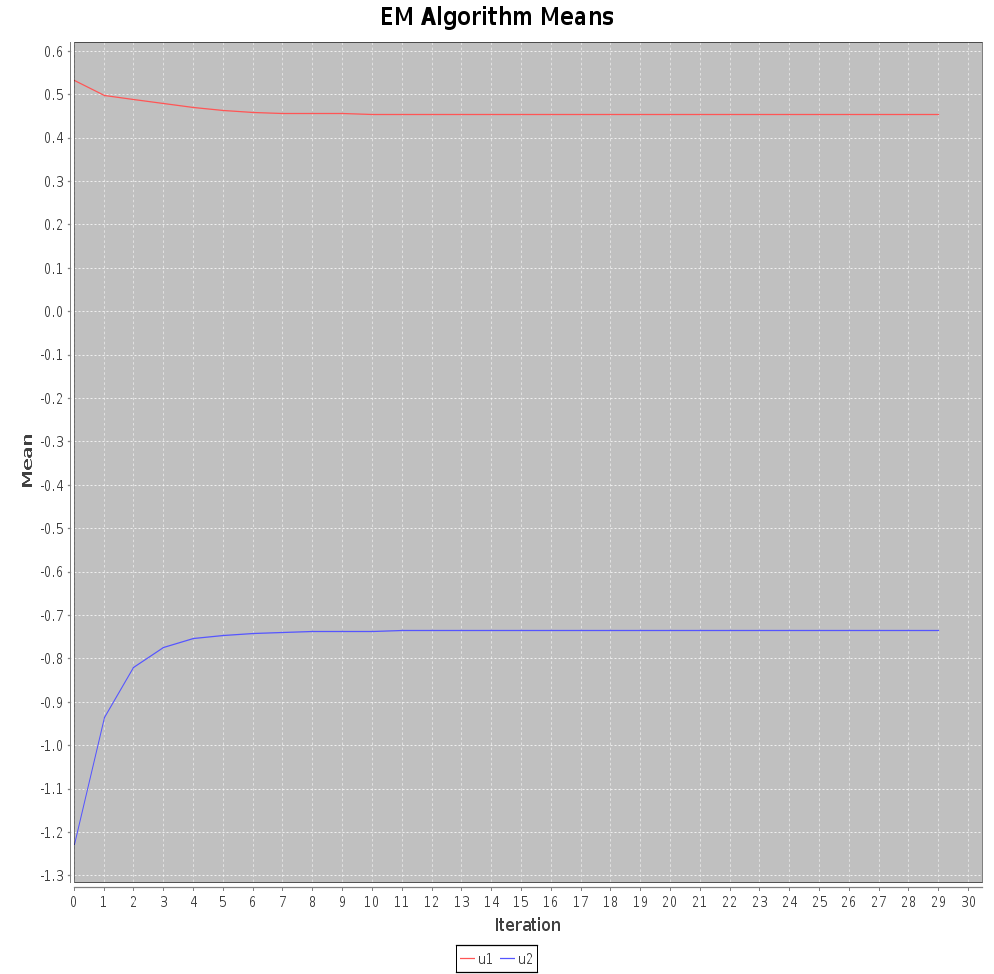
\includegraphics[width=0.7\textwidth]{em-means.png}
\caption{Evolution of Mean Estimates using EM Algorithm}
\label{fig1}
\end{figure}

\begin{figure}
\centering
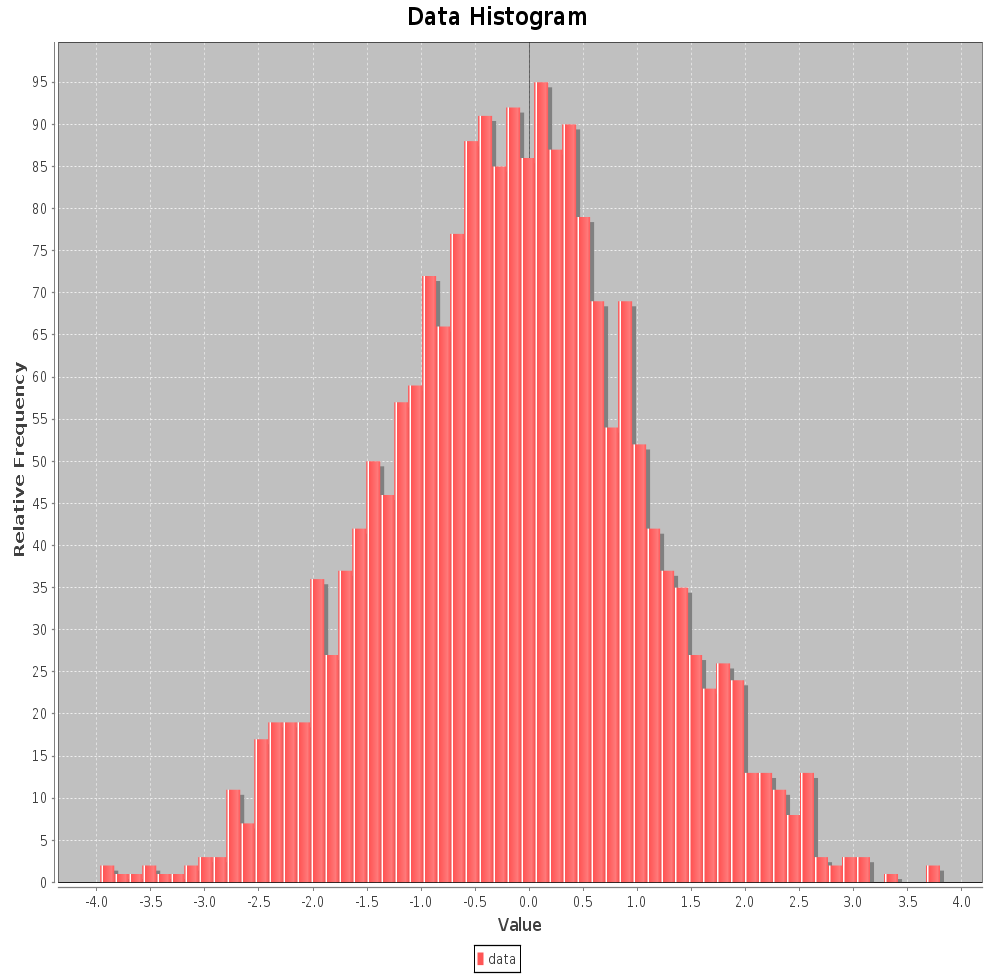
\includegraphics[width=0.7\textwidth]{em-data.png}
\caption{EM Data Set Geoffrey.txt}
\label{fig2}
\end{figure}


\begin{thebibliography}{9}

\bibitem{cpl}
  Tom M. Mitchell,
  \emph{Machine Learning},
  WCB McGraw-Hill, Boston,
  1997.

\end{thebibliography}

\end{document}
